\documentclass[a4paper,10pt]{article}
\usepackage[utf8]{inputenc}
\usepackage{listings}
\usepackage{color}
\usepackage{graphicx}
\lstset{ %
  language=R,                     % the language of the code
  basicstyle=\footnotesize,       % the size of the fonts that are used for the code
  numbers=left,                   % where to put the line-numbers
  numberstyle=\tiny\color{gray},  % the style that is used for the line-numbers
  stepnumber=1,                   % the step between two line-numbers. If it's 1, each line
                                  % will be numbered
  numbersep=5pt,                  % how far the line-numbers are from the code
  backgroundcolor=\color{white},  % choose the background color. You must add \usepackage{color}
  showspaces=false,               % show spaces adding particular underscores
  showstringspaces=false,         % underline spaces within strings
  showtabs=false,                 % show tabs within strings adding particular underscores
  frame=single,                   % adds a frame around the code
  rulecolor=\color{black},        % if not set, the frame-color may be changed on line-breaks within not-black text (e.g. commens (green here))
  tabsize=2,                      % sets default tabsize to 2 spaces
  captionpos=b,                   % sets the caption-position to bottom
  breaklines=true,                % sets automatic line breaking
  breakatwhitespace=false,        % sets if automatic breaks should only happen at whitespace
  title=\lstname,                 % show the filename of files included with \lstinputlisting;
                                  % also try caption instead of title
  keywordstyle=\color{blue},      % keyword style
  commentstyle=\color{dkgreen},   % comment style
  stringstyle=\color{mauve},      % string literal style
  escapeinside={\%*}{*)},         % if you want to add a comment within your code
  morekeywords={*,...}            % if you want to add more keywords to the set
}
\definecolor{dkgreen}{rgb}{0,0.6,0}
\definecolor{gray}{rgb}{0.5,0.5,0.5}
\definecolor{mauve}{rgb}{0.58,0,0.82}
%opening
\title{Pattern Recognition and Data Mining HW3}
\author{Kevin Aloysius and Nicki Bi}

\begin{document}

\maketitle

\section{Solution 9.7.3 (a)}
\begin{lstlisting}[language=R]
# Solution (a)
x1 <- c(3, 2, 4, 1, 2, 4, 4)
x2 <- c(4, 2, 4, 4, 1, 3, 1)
colors <- c("red","red","red","red","blue","blue","blue")
plot(x1,x2, col = colors, xlim = c(0,5), ylim = c(0,5), main = "Solution 9.7.3(a)")
\end{lstlisting}
\begin{center}
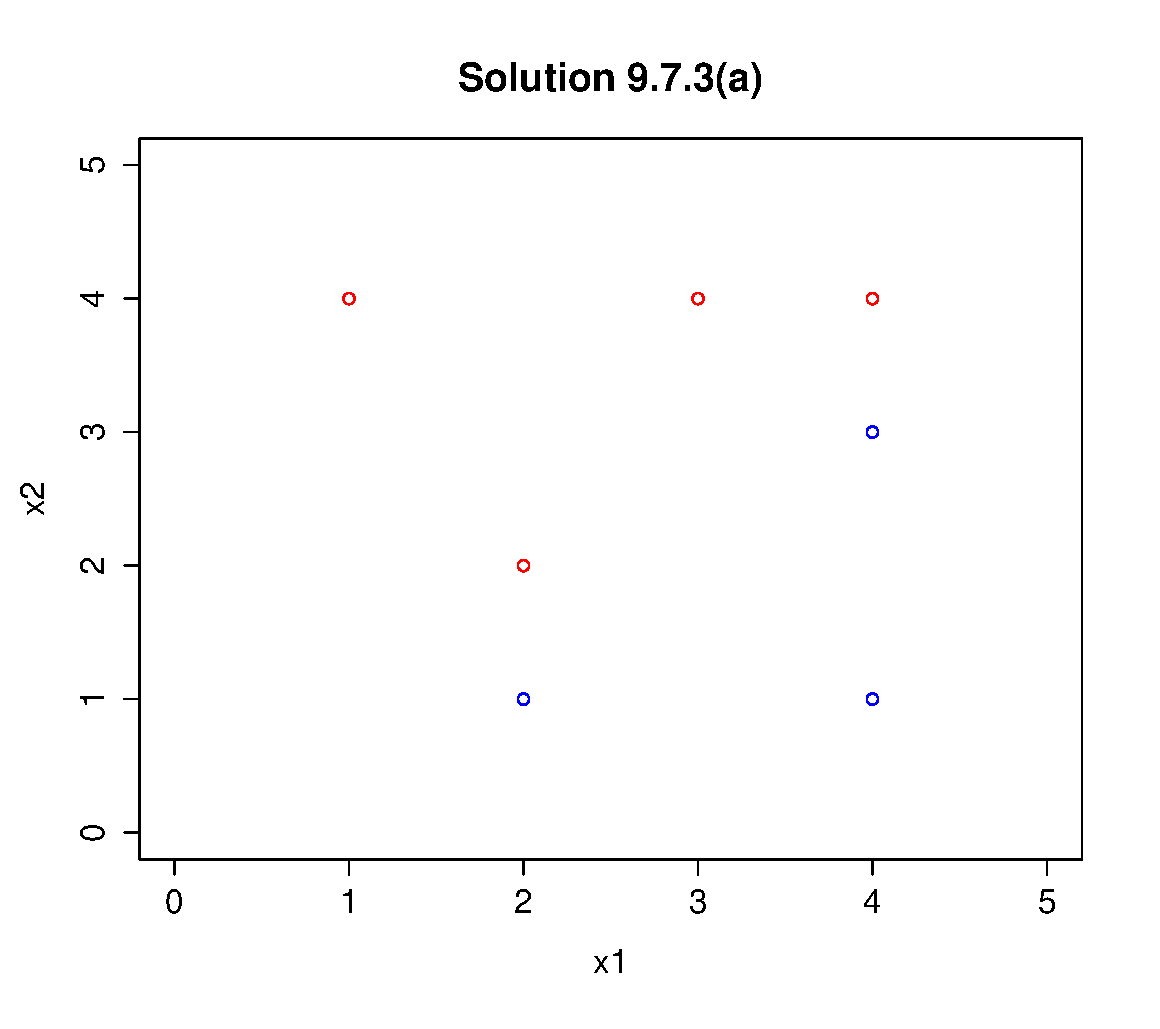
\includegraphics[scale=0.70]{first}
\end{center}

\section{Solution 9.7.3 (b)}
\begin{lstlisting}[language=R]
#Solution (b)
plot(x1,x2, col = colors, xlim = c(0,5), ylim = c(0,5), main = "Solution 9.7.3(b)", abline(-0.5,1))
\end{lstlisting}
\begin{center}
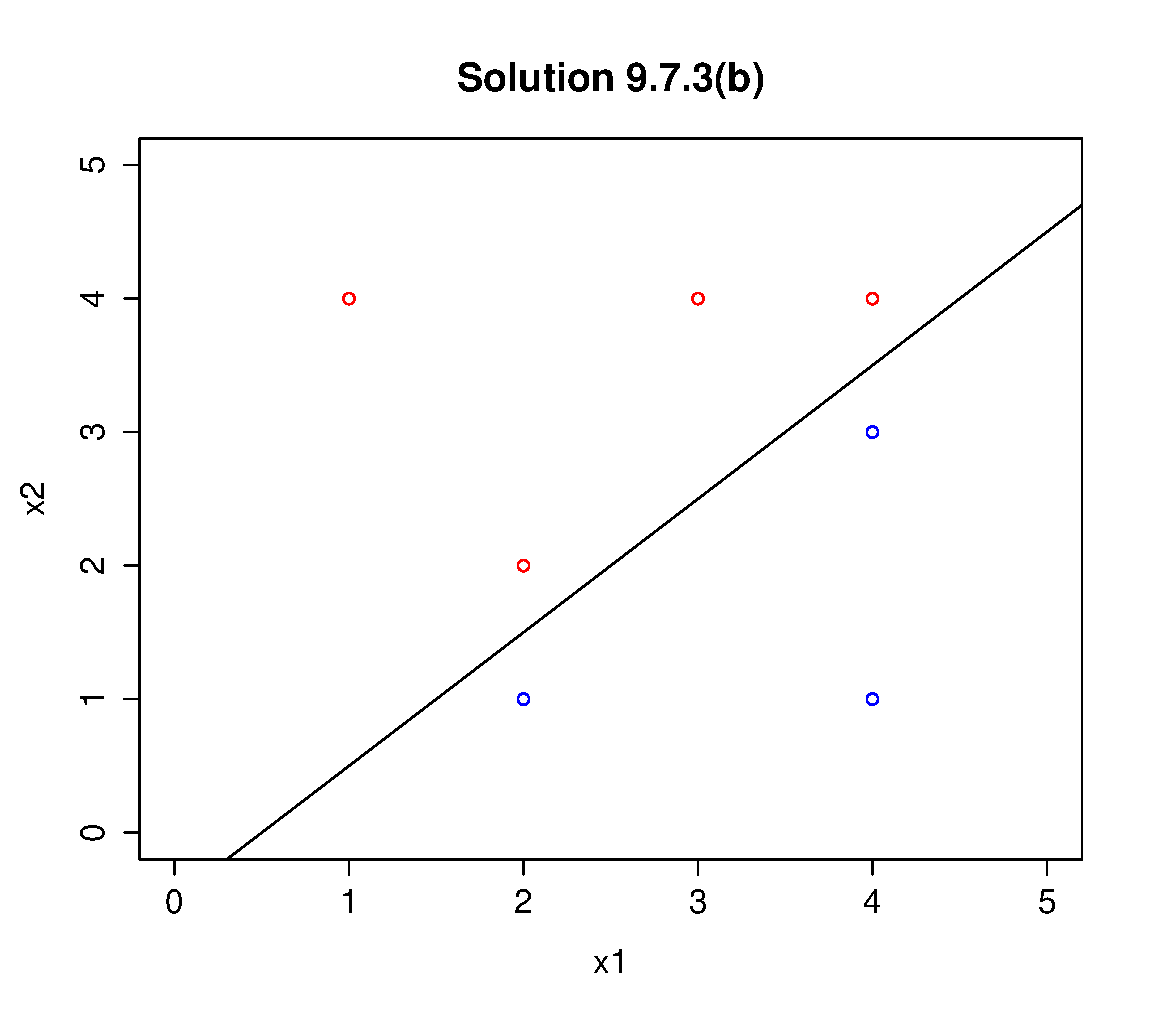
\includegraphics[scale=0.70]{second}
\end{center}
The Maximal Marginal Classifier is the hyperplane that is passing through the points $(2,1.5)$ and $(4,3.5)$.\newline
The equation of the hyperplane in $\beta_0 + \beta_1X_1 + \beta_2X_2$ form \newline is $0.5-X_1+X_2=0$
\newpage
\section{Solution 9.7.3 (c)}
The Classification Rule for the Maximum Marginal Classifier is as follows,\newline ``Classify to Red if $0.5-X_1+X_2>0$ and classify to Blue otherwise''

\section{Solution 9.7.3 (d)}
\begin{lstlisting}[language=R]
#Solution (e)
plot(x1, x2, col = colors, xlim = c(0, 5), ylim = c(0, 5), main = "Solutions 9.7.3(e)")
abline(-0.5, 1)
abline(-1, 1, lty = 2)
abline(0, 1, lty = 2)
arrows(2, 1, 2, 1.5)
arrows(2, 2, 2, 1.5)
arrows(4, 4, 4, 3.5)
arrows(4, 3, 4, 3.5)
\end{lstlisting}
\begin{center}
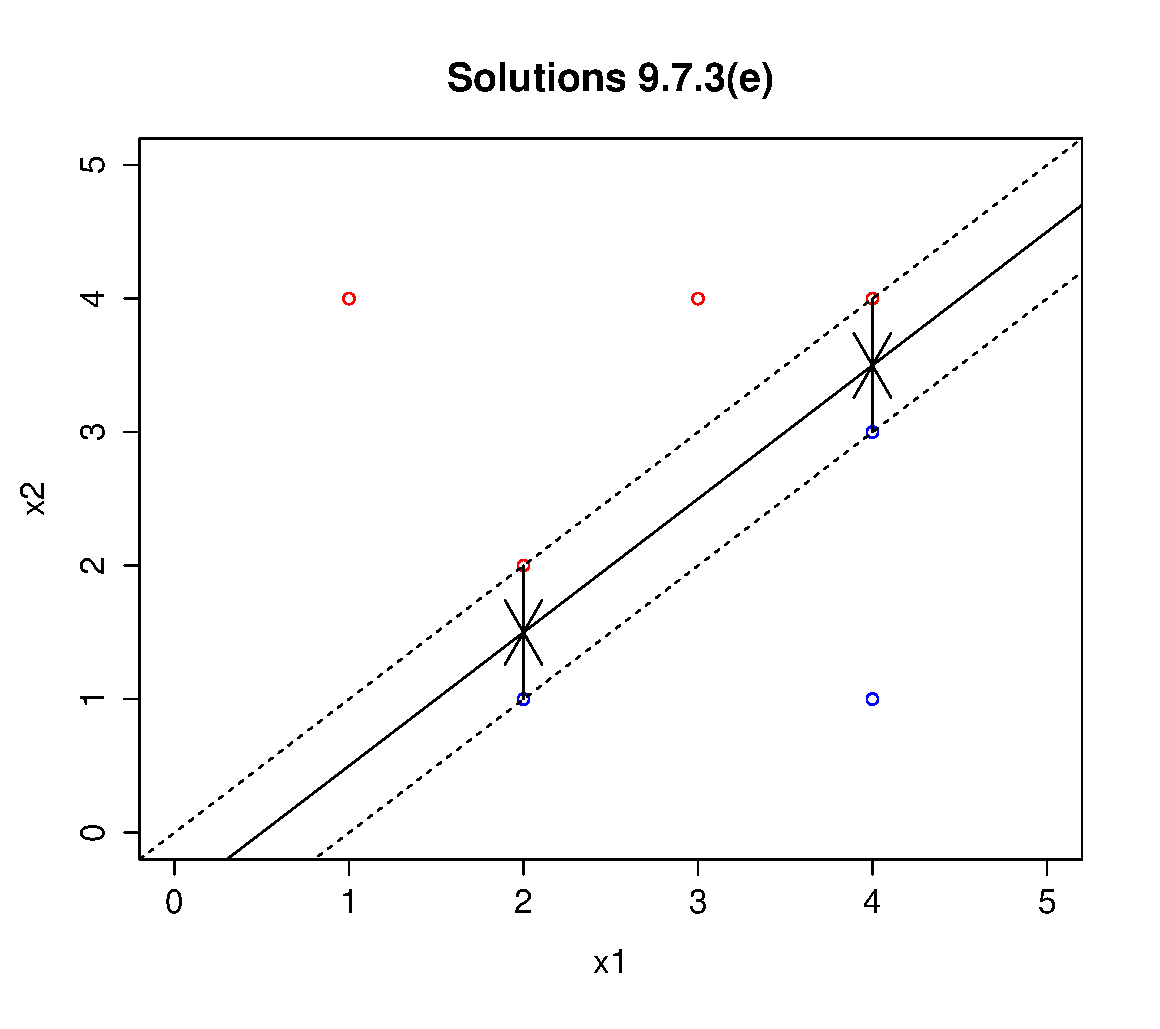
\includegraphics[scale=0.70]{support}
\end{center}

\section{Solution 9.7.3 (e)}
A slight movement of the $7^{th}$ observation would not affect the Maximal Margin Hyperplane because the $7^{th}$ observation which is $(4,1)$ is well beyond the
margin of the support vectors and therefore it's movement won't affect the margin of the support vector thereby not affecting the Maximal
Margin Hyperplane.

\section{Solution 9.7.3 (g)}
\begin{lstlisting}[language=R]
#Solution (g)
plot(x1, x2, col = colors, xlim = c(0, 5), ylim = c(0, 5), main = "Solution 9.7.3(g)")
abline(-0.85, 1)
\end{lstlisting}
\begin{center}
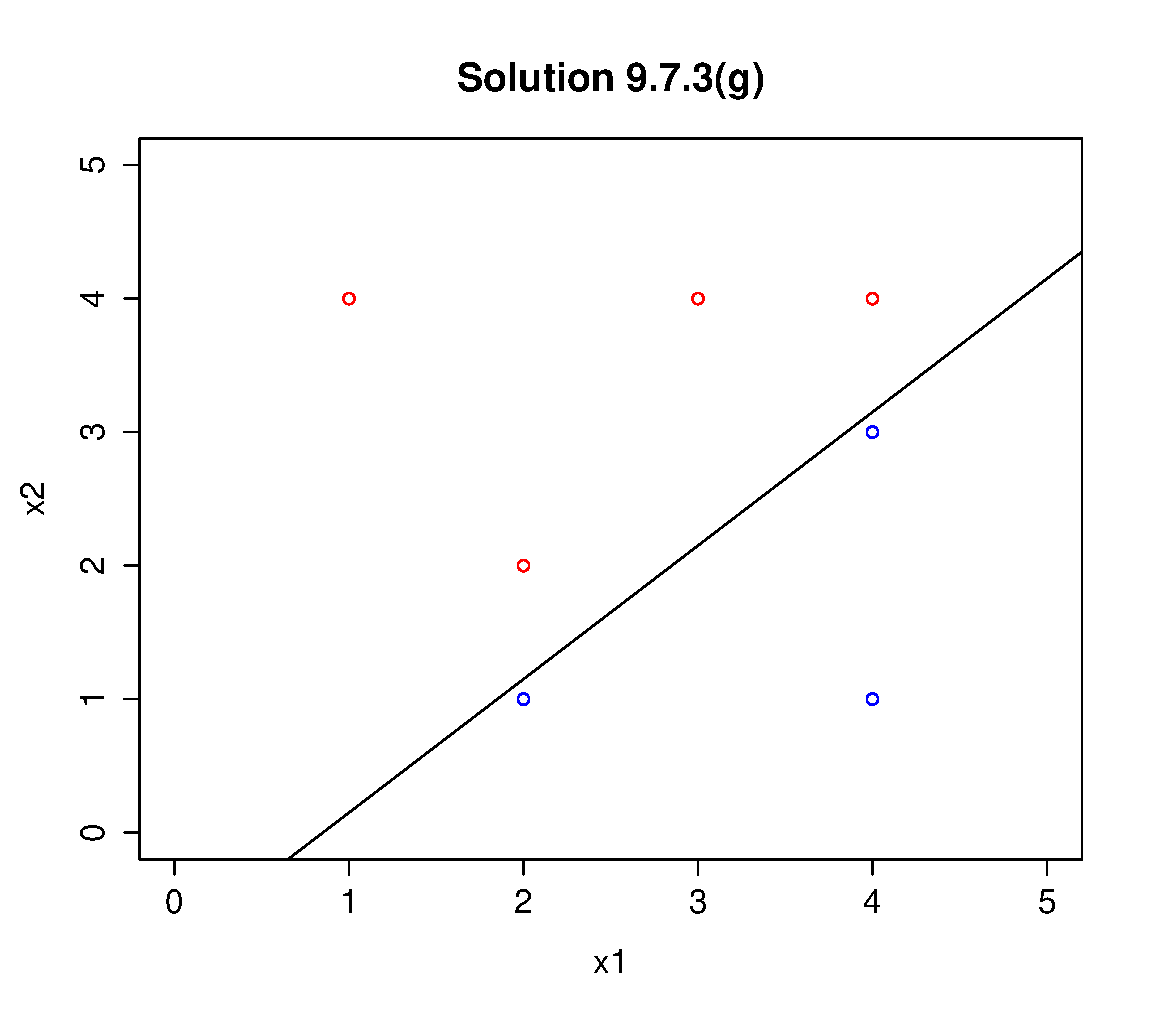
\includegraphics[scale=0.70]{not_optimal}
\end{center}
The equation of the hyperplane in $\beta_0 + \beta_1X_1 + \beta_2X_2$ form \newline is $-0.85-X_1+X_2=0$

\section{Solution 9.7.3 (h)}
\begin{lstlisting}[language=R]
#Solution (h)
plot(x1, x2, col = colors, xlim = c(0, 5), ylim = c(0, 5), main = "Solution 9.7.3(h)")
points(c(3), c(2), col = c("red"))
\end{lstlisting}
\begin{center}
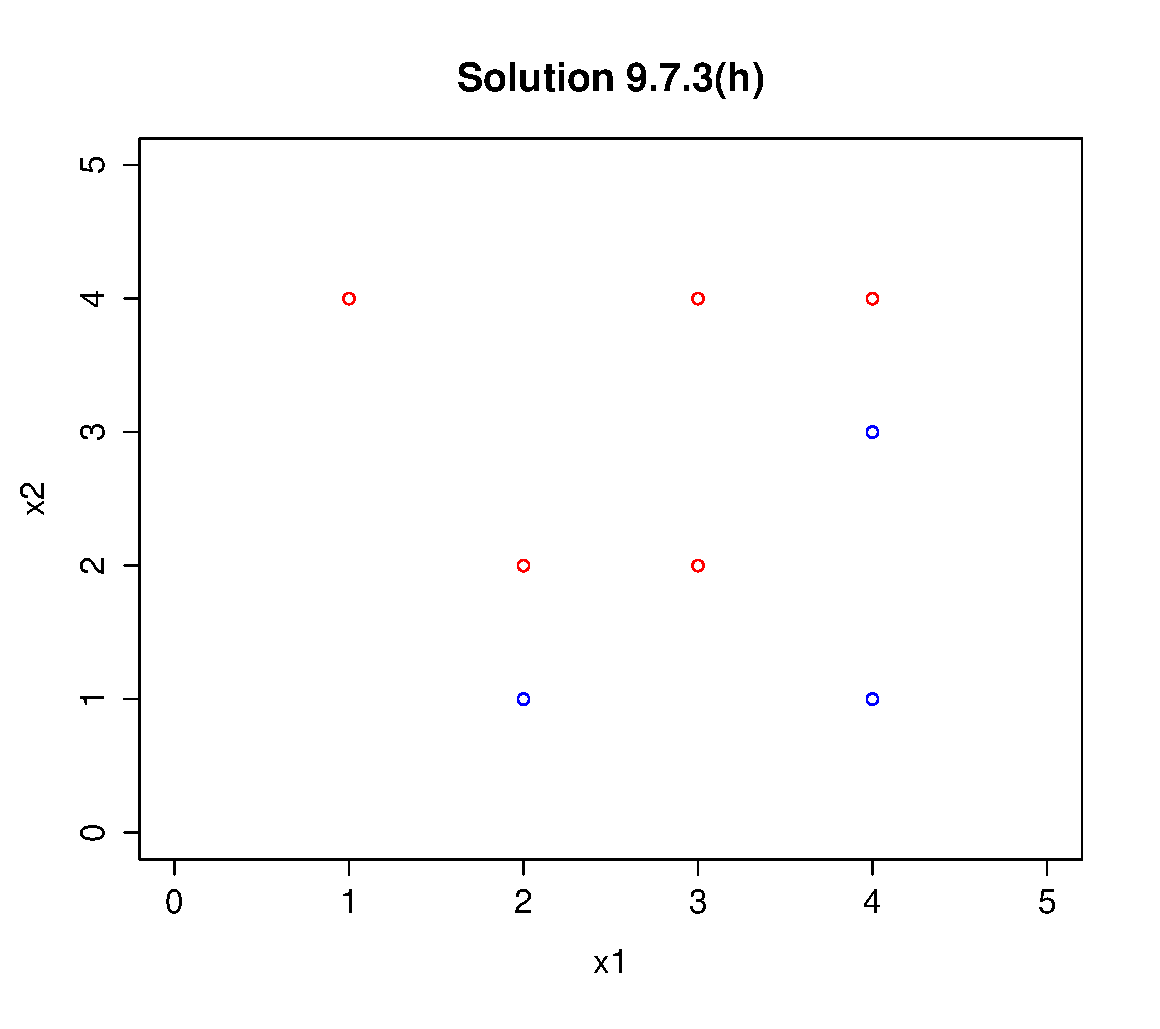
\includegraphics[scale=0.70]{additional_obs}
\end{center}
\end{document}